\documentclass[twocolumn, a4paper, 10pt]{article}

%= PAGE/CONTENT SIZE
\usepackage[margin={1cm,2.5cm}]{geometry}
\setlength{\columnsep}{0.5cm}

%= FONT FAMILY
\fontfamily{ptm}\selectfont

%= FIGURES & GRAPHICS
\usepackage{graphicx}
\graphicspath{{figures/}}
\usepackage{floatrow}

%= BIBLIOGRAPHY
\usepackage[backend=bibtex,style=alphabetic,bibencoding=ascii,sorting=ynt]{biblatex}
\addbibresource{bibliography}

%= BETTER MATH
\usepackage{amssymb}
\usepackage{amsmath}
\usepackage{pst-node}
\usepackage{cases}

%= LOREM IPSUM
\usepackage{lipsum}

%%%%%%%%%%%%%%%%%%%%%%%%%%%%%%%%%%%%%%%%%%%%%%%%%%%%%%%%%%%%%%%%%%%%%%%%%%%%%%%%%
%% FIXES
%%%%%%%%%%%%%%%%%%%%%%%%%%%%%%%%%%%%%%%%%%%%%%%%%%%%%%%%%%%%%%%%%%%%%%%%%%%%%%%%%

% #1 : DOT AFTER SECTION
\usepackage{titlesec}
\titlelabel{\thetitle. }

% #2 : TIKZ PACKAGES
\usepackage{tikz}
\usepackage{xcolor}
\usepackage{framed}
\usepackage{etoolbox}
\usepackage{smartdiagram}

\usetikzlibrary{arrows,positioning}
\usetikzlibrary{decorations}
\usetikzlibrary{decorations.pathreplacing}
\usetikzlibrary{shapes.arrows,chains}
\usetikzlibrary{fit,shapes}
\usetikzlibrary{calc}

% #3 : TIKZ CONFIGURATION
\tikzset{
    >=stealth',
    punkt/.style={
           rectangle,
           rounded corners,
           draw=black, very thick,
           text width=6.5em,
           minimum height=2em,
           text centered},
    pil/.style={
           ->,
           thick,
           shorten <=2pt,
           shorten >=2pt,}
}

% #4 : CODE/SNIPPETS APPENDIX
\usepackage{algorithm2e}
\usepackage{listings}
\lstset{language=C}

% #5 : LST CONFIGURATION
\lstdefinestyle{codeAppendix}{
  language=C,
  numbers=left,
  stepnumber=1,
  numbersep=10pt,
  tabsize=2,
  showspaces=false,
  showstringspaces=false,
  frame=single,
  basicstyle=\ttfamily\footnotesize,
}

% #6 : LIST MARGIN
\usepackage{enumitem}
\setlist[itemize]{leftmargin=4mm}

% #7 : THEOREM
\newtheorem{theorem}{Theorem}[section]
\newtheorem{corollary}{Corollary}[theorem]
\newtheorem{lemma}[theorem]{Lemma}

% #8 : QUOTES
\usepackage{csquotes}

%%%%%%%%%%%%%%%%%%%%%%%%%%%%%%%%%%%%%%%%%%%%%%%%%%%%%%%%%%%%%%%%%%%%%%%%%%%%%%%%%
%% VARIABLES
%%%%%%%%%%%%%%%%%%%%%%%%%%%%%%%%%%%%%%%%%%%%%%%%%%%%%%%%%%%%%%%%%%%%%%%%%%%%%%%%%

%= TITLE
\title{\fontsize{18.5}{14.4}\textbf{\MakeUppercase{Chaos Machine: Different Approach to the Application and Significance of Numbers}}}

%= AUTHOR
\author{
  Maciej A. Czyzewski\\
  \texttt{mail@maciejczyzewski.me}
}

\begin{document}

\maketitle

%%%%%%%%%%%%%%%%%%%%%%%%%%%%%%%%%%%%%%%%%%%%%%%%%%%%%%%%%%%%%%%%%%%%%%%%%%%%%%%%%
%%%%%%%%%%%%%%%%%%%%%%%%%%%%%%%%%%%%%%%%%%%%%%%%%%%%%%%%%%%%%%%%%%%%%%%%%%%%%%%%%
%%                            BEGIN OF DOCUMENT                                %%

\noindent\textbf{Abstract.} In this paper we describe a theoretical model of \underline{chaos machine}, which combines the benefits of hash function and pseudo-random function, forming flexible \textit{one-way} \underline{push-pull interface}. It presents the idea to create a universal tool (design pattern) with modular design and customizable parameters,   that can be applied    where   \textit{randomness} and \textit{sensitiveness} is needed (random oracle), and    where   appropriate construction determines case of application and selection of parameters provides preferred properties and security level. Machine can be used to implement many cryptographic primitives, including cryptographic hashes, message authentication codes and pseudo-random number generators.
Additionally, document includes sample implementation of chaos machine named Naive Czyzewski Generator, abbreviated NCG, that passes all the Dieharder, NIST and TestU01 test sets. Algorithm was designed and evaluated to be a cryptographically strong, inasmuch as indistinguishable from a uniform random function. The generator was developed to work as cryptographically secure pseudo-random number generator, collision resistance hash function or a cryptographic module. One can target a given period length by choosing the appropriate space parameter, i.e., for a given parameter $m$, algorithm is claimed to have period between $2^{8m}$ to $2^{16m}$.
\newline\newline
\noindent\textbf{Keywords.} chaos machine $\cdot$ dynamical system $\cdot$ chaotic behavior $\cdot$ randomness $\cdot$ control theory $\cdot$ chaotic map $\cdot$ pseudo-random function $\cdot$ push-pull interface

%%%%%%%%%%%%%%%%%%%%%%%%%%%%%%%%%%%%%%%%%%%%%%%%%%%%%%%%%%%%%%%%%%%%%%%%%%%%%%%%%
%% INTRODUCTION
%%%%%%%%%%%%%%%%%%%%%%%%%%%%%%%%%%%%%%%%%%%%%%%%%%%%%%%%%%%%%%%%%%%%%%%%%%%%%%%%%

\section*{Introduction}

A lot of research has gone into chaos and randomness theory. Development in computer software and applications continues to be very dynamic. Each software problem requires different tools and algorithms to solve it effectively and achieve best results. As a consequence, we witness the announcement of new projects in quick succession with multiple updates. The engineer's problem is how to decide which method will suit his needs best.

Random numbers have been one of the most useful objects in statistics, computer science, cryptography, modeling, simulation, and other applications though it is very difficult to construct true randomness. Many applications of randomness have led to the development of several methods for generating random data. The generation of pseudo-random numbers is an important and common task in computer programming. Cryptographers design algorithms such as RC4 and DSA, and protocols such as SET and SSL, with the assumption that random numbers are available.

Hash is the term basically originated from computer science where it means chopping up the arbitrary length message into fixed length output. Hash tables are popular data structures for storing key-value pairs. A hash function is used to map the key value to array index, because it has numerous applications from indexing, with hash tables and bloom filters; to spell-checking, compression, password hashing and cryptography. They are used in many different kinds of settings and accordingly their security requirement changes.

Hash functions were designed for uniqueness, while pseudo-random functions for randomness\footnote{In practice, hash functions are chosen to spread hash values uniformly (pseudo-randomly). However, some techniques of hashing does not require this principle.}. There is a tendency for people to avoid learning anything about such subroutines \cite{Knuth1973}; quite often we find that some old method that is comparatively unsatisfactory has blindly been passed down from one programmer to another, and today's users have no understanding of its limitations. Therefore, appears the idea to create a universal tool (design pattern) with modular design and customizable parameters, that can be applied where \textit{randomness} and \textit{sensitiveness} is needed (random oracle), and where appropriate construction determines case of application and selection of parameters provides preferred properties and security level. It should be so easy to use that an intelligent, careful programmer with no background in cryptography has some reasonable chance of using such tool in secure way.

In this paper we describe a theoretical model of chaos machine, which combines the benefits of hash function and pseudo-random function, forming flexible \textit{one-way}\footnote{One-way functions are easy to compute but it is very difficult to compute their inversed functions.} push-pull interface, where the construction and selection of parameters determines usage. It generates sequences of pseudo-random numbers that are unique and sensitive to the initial conditions and inputs. Therefore, machine can be used to implement many cryptographic primitives, including cryptographic hashes, message authentication codes and pseudo-random number generators.

%%%%%%%%%%%%%%%%%%%%%%%%%%%%%%%%%%%%%%%%%%%%%%%%%%%%%%%%%%%%%%%%%%%%%%%%%%%%%%%%%
%%%%%%%%%%%%%%%%%%%%%%%%%%%%%%%%%%%%%%%%%%%%%%%%%%%%%%%%%%%%%%%%%%%%%%%%%%%%%%%%%
%% PART 1

\twocolumn[
  \begin{@twocolumnfalse}
  \clearpage
  \part{Definition and Analysis of the Model}
  \vspace*{1.5cm}
  \end{@twocolumnfalse}
]

%%%%%%%%%%%%%%%%%%%%%%%%%%%%%%%%%%%%%%%%%%%%%%%%%%%%%%%%%%%%%%%%%%%%%%%%%%%%%%%%%
%% OVERVIEW
%%%%%%%%%%%%%%%%%%%%%%%%%%%%%%%%%%%%%%%%%%%%%%%%%%%%%%%%%%%%%%%%%%%%%%%%%%%%%%%%%

\section{Overview}

Chaos theory started more than thirty years ago and changed our world view regarding the role of randomness and determinism, these theories present some interesting aspects in cryptography: \begin{itemize} \item Chaotic systems are highly sensitive to initial conditions and exhibits chaotic behavior. The main characteristics of chaotic systems make them intuitively interesting for their application in cryptography. Edward Lorenz used to say ``Chaos: When the present determines the future, but the approximate present does not approximately determine the future.''.
\item Randomness is the lack of pattern or predictability in events, a phenomenon located at a single point in spacetime. A pseudo-random process is a process that appears to be random but is not. Pseudo-random sequences typically exhibit statistical randomness while being generated by an entirely deterministic causal process. \end{itemize}

\subsection{Concept}
\label{ssec:concept}

Idea was to create simple model (design pattern) containing several elements, that lets programmer to create own constructions and tools where \textit{randomness} and \textit{sensitiveness} is needed (random oracle). These main assumptions are presented as:

\begin{itemize}

\item\textbf{Diffusion}: a small difference in the input produces a very different output.

\item\textbf{Deterministic Pseudo-randomness}: a deterministic procedure that produces pseudo-randomness.

\item\textbf{Algorithmic Complexity}: a simple algorithm that produces highly complex outputs.

\end{itemize}

Where selection of parameters provides preferred properties and security level. Therefore, machine contains three external variables: \textit{initial secret key}, \textit{time parameter}, and \textit{space parameter}.

\begin{itemize}

\item\textbf{Initial Secret Key} (Starting Variable). Is a fixed-size input to a chaos machine that is typically required to be random or pseudo-random. Setting the initial secret key is an example of using machine as the MAC\footnote{A message-authentication code (MAC) produces a tag $t$ from a message $m$ and a secret key $k$. The security goal is for an attacker, even after seeing tags for many messages (perhaps selected by the attacker), to be unable to guess tags for any other messages.} algorithm.

\item\textbf{Time Parameter} (Time Cost). That determines the number of rounds of computation that machine performs. The larger the time parameter, the longer the output computation will take. As computational power increases, users can increase this time parameter to keep the number of wall-clock seconds required to compute each sequence near-constant.

\item\textbf{Space Parameter} (Memory Cost). Defines the number of dynamical systems to be used in the machine. Concomitantly indicates how many bytes of working space the buffer will require during its computation, because each system needs his own space.

\end{itemize}

Model contains dynamical system of \textit{push-pull-reset functions} and \textit{buffer space}. Components below are forming machine interface:

\begin{itemize}

\item\textbf{Push Function} (Input). Is primarily the input function, it absorbs bit string (typically 32 bits or 16 bits value, relatively small) and uses in system evaluation (control theory, it will be discussed later).

\item\textbf{Pull Function} (Output). It contains chaotic map and construction of pseudo-random functions, which can be freely replaced. The output of pull function is a bit string of fixed length (e.g., 32 or 16 bits).

\item\textbf{Reset Function} (Reset). This function clears the buffer. After this, operation machine is in the initial state.

\end{itemize}

Applying our recommendations, programmer can build effective machine for wide range of applications. An example is described in the second part of this document.

%%%%%%%%%%%%%%%%%%%%%%%%%%%%%%%%%%%%%%%%%%%%%%%%%%%%%%%%%%%%%%%%%%%%%%%%%%%%%%%%%
%% MODEL
%%%%%%%%%%%%%%%%%%%%%%%%%%%%%%%%%%%%%%%%%%%%%%%%%%%%%%%%%%%%%%%%%%%%%%%%%%%%%%%%%

\section{Model}

\begin{figure}[ht]
  \centering
  \floatbox[{\capbeside\thisfloatsetup{capbesideposition={right,top},capbesidewidth=4cm}}]{figure}[\FBwidth]
  {\vspace*{-38.5pt}\caption{Machine contains 3 main elements: push function, buffer space, pull function. Its initialized by tuple $(K, t, m)$, where $K$ is initial secret key, $t$ is time parameter and $m$ is space parameter.}\label{fig:machine-diagram}}
  {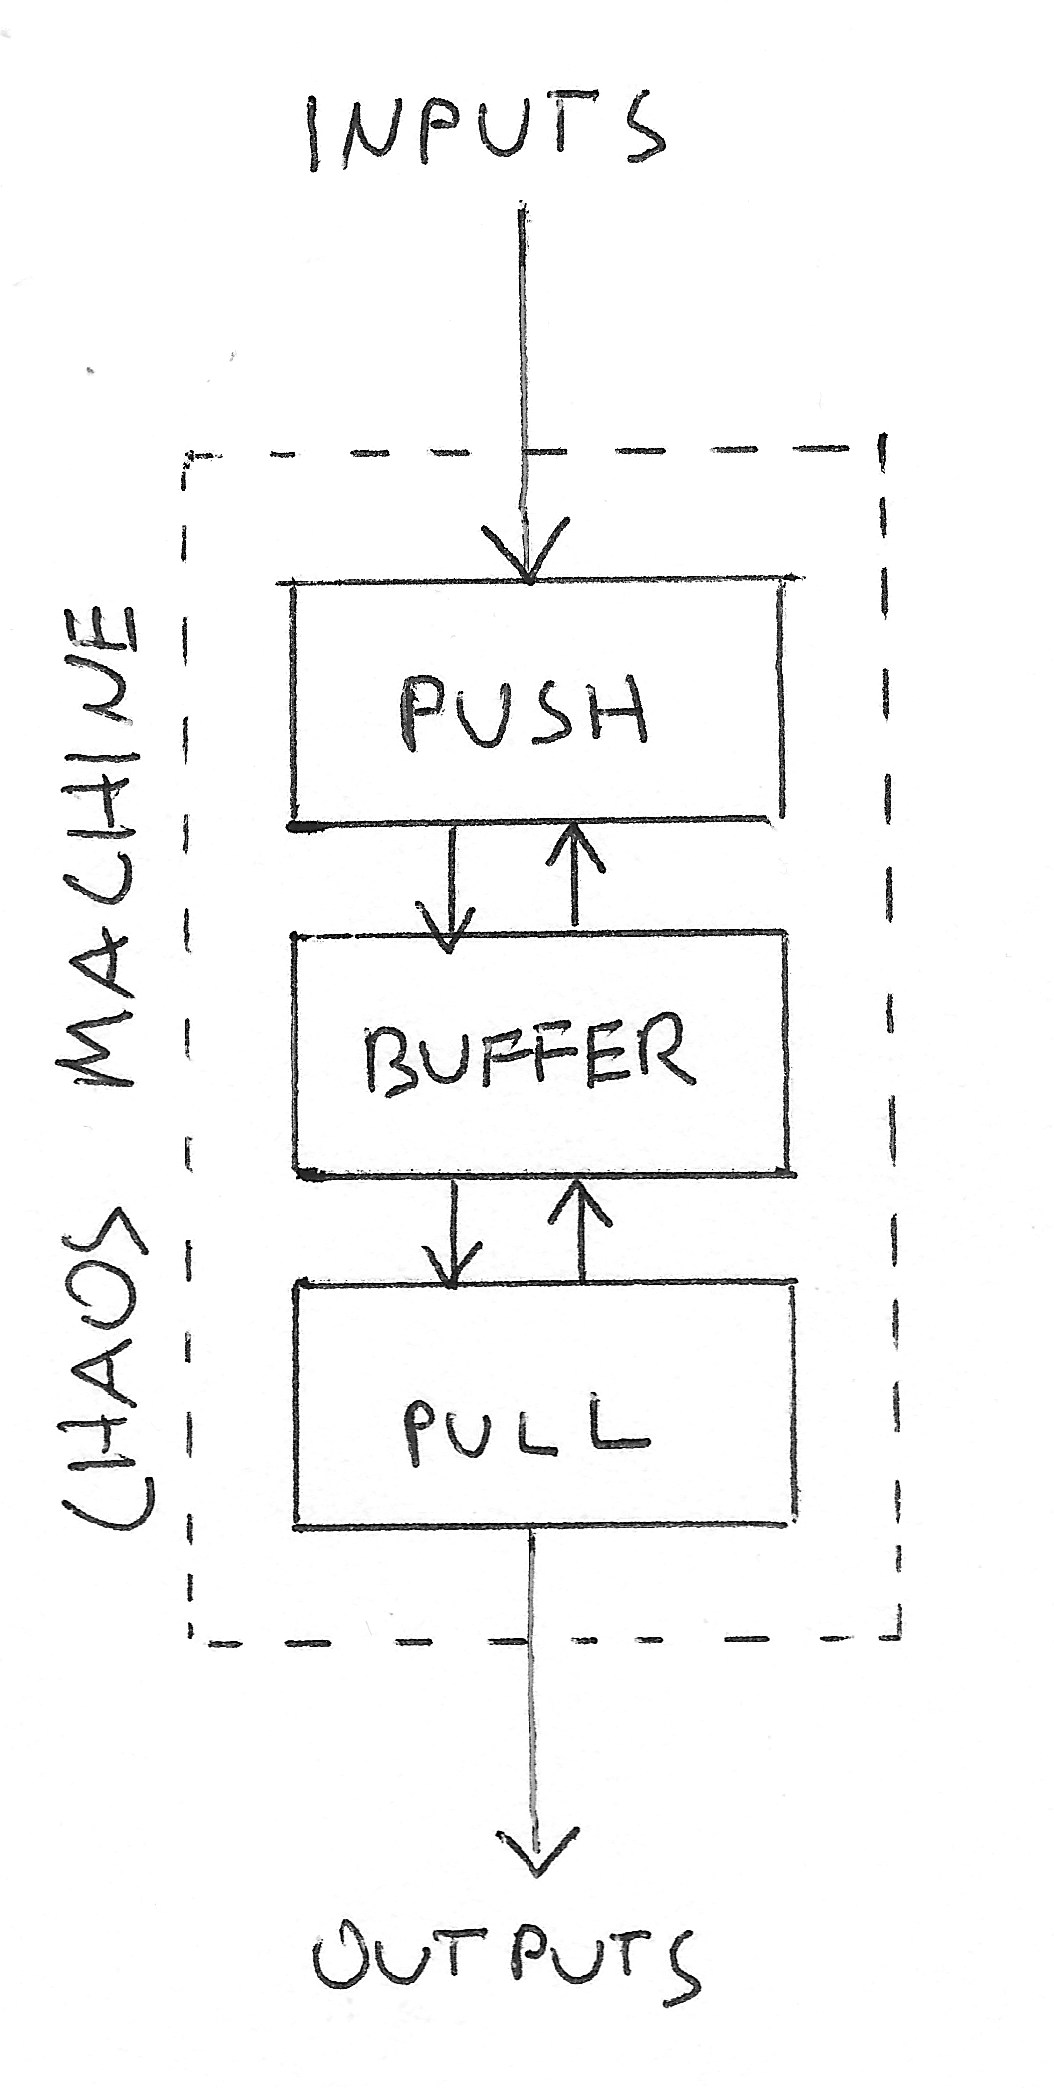
\includegraphics[width=3.25cm]{machine-diagram}}
\end{figure}

%%%%%%%%%%%%%%%%%%%%%%%%%%%%%%%%%%%%%%%%%%%%%%%%%%%%%%%%%%%%%%%%%%%%%%%%%%%%%%%%%
%% DYNAMICAL SYSTEM

\subsection{Dynamical System}

Chaos is a non-periodic, long-term non-predictive behavior that can be generated by certain nonlinear dynamical systems \cite{Opac-b1101628}. The chaotic systems are inherently deterministic given the initial state of the system. The chaotic behavior is a result of the exponential sensitivity of the system to the initial state that can not be exactly determined in practice.

\subsubsection{Discrete \& Continues}

There is two main models of evolution law \cite{Viana2001}. The first one corresponds to transformations $f : M \to M$ on a space $M$, the points of which describe the different states of the system. The orbit of each $x_0 \in M$ is the sequence $(x_n)_n$ defined by $x_n = f(x_{n-1})$ for $n > 1$.

Another model are continues-time flows $f^t : M \to M$, $t \in \mathbb{R}$, that is, one-parameter families of transformations satisfying $f^{t+s} = f^t \circ f^s$ for $t, s \in \mathbb{R}$, and $f^0 = id$. The orbit of $x_0 \in M$ is the curve $x_t = f^t(x_0)$, where $t \in \mathbb{R}$. Assuming the flow depends smoothly on time $t$, there is an associated vector field $F$ on $M$, defined by: $$F(x) = \frac{d}{dt} f^t(x) \vert_{t=0}$$

\subsubsection{Computer Limitations}

A computer is a finite state machine that may be viewed as a discrete system. As in the discrete-time case, the solutions for the function $f$ are no longer curves, but points that hop in the phase space. The orbits are organized in curves, or fibers, which are collections of points that map into themselves under the action of the map. However, some methods have been developed to represent real-world continuous systems as discrete systems \cite{2014JChPh.140c4105T}.

\subsubsection{Transition}

In our model, each map $f$, chaotic or not, will be called a position \textit{transition function} of dynamical system designated as $T$. To watch out for the multidimensionality of point $x$, we will write it as a vector $\vec{x}$.

\begin{theorem}
[Coordinate Function]
\label{coordinate-function}\hfill\break
If $\vec{x} = (x_1, \dots, x_n) \in \mathbb{R}^n$ is a point in the $n$-space then we define the $i$-th coordinate function $p_i : \mathbb{R}^n \to \mathbb{R}$ as $p_i(\vec{x}) = x_i$
\end{theorem}

\begin{theorem}
[Transition Function]
\label{transition-function}\hfill\break
More generally, transition function is a map from one position to another. In the theory of dynamical systems, a map denotes an evolution function used to create discrete dynamical systems. Using definition of point from \ref{coordinate-function}, transition function $T : \mathbb{R}^n \to \mathbb{R}^n$ is defined: $$T(\vec{x}) = T([x_1, \dots, x_n]) = [p_1, \dots, p_n]$$

Then, transition in dynamical system is described as: $$\vec{x_i} = T(\vec{x_{i-1}})$$

This map takes a point $\vec{x_{i-1}} = (x_1, \dots, x_n)$ in the space and maps it to a new point $\vec{x_i} = (p_1(\vec{x_{i-1}}), \dots, p_n(\vec{x_{i-1}}))$.
\end{theorem}

In dynamical system's theory, the \textit{Gingerbreadman map} is a chaotic two-dimensional map which was studied by R. Devaney \cite{Devaney1984} since 1984. It is given by the piecewise linear transformation: $$\begin{cases} x_{n+1} = 1 - y_n + |x_n| \\ y_{n+1} = x_n \end{cases}$$

Using theorem from \ref{coordinate-function}, it can be written as set of coordinate functions: \begin{gather} p_1(\vec{x}) = 1 - x_2 + |x_1| \\ p_2(\vec{x}) = x_1 \end{gather}

Then, \textit{Gingerbreadman map} is equivalent to the transition $T : \mathbb{R}^2 \to \mathbb{R}^2$ given by: $$\vec{x_n} = T(\vec{x_{n-1}}) = T([x_1, x_2]) = [p_1, p_2] = [1 - x_2 + |x_1|, x_1]$$

This map takes a point $\vec{x_{n-1}} = (x_1, x_2)$ in the plane and maps it to a new point $\vec{x_n} = (p_1(\vec{x_{n-1}}), p_2(\vec{x_{n-1}}))$. Coordinate function (1) and (2) calculates coordinates of the next state in chaotic map.

\begin{theorem}
[Dynamical System]
\label{dynamical-system}\hfill\break
In general sense, dynamical system $\phi: t \times \mathbb{R}^n \to \mathbb{R}^n$ where $t$ is time (for discrete $t = \mathbb{Z}$ or $t = \mathbb{N}$), can be described as: $$\vec{x_i} = T(\vec{x_{i-1}})$$

Using the \ref{transition-function} theorem and definition of evolution function $\phi$, superscript of function $T$ defines time (or iteration): $$\phi_i(\vec{x}) := T(\phi_{i-1}(\vec{x})) = T^i(\vec{x})$$

Evolution (trace) of discrete dynamical system from the initial state $\vec{x_0} \in \mathbb{R}^n$: $$\vec{x_0} = T^0(\vec{x_0}) \to T^1(\vec{x_0}) \to T^2(\vec{x_0}) \to T^3(\vec{x_0}) \to \dots$$
\end{theorem}

\subsubsection{Vector of Systems}
\label{sssec:buffer-space}

\begin{figure}
\begin{verbatim}
   ............................................
   .                  BUFFER                  .
   .         ...                              .
   .        . 1 .  2    3   ...   m           .
   .     ../  / \ ........                    .
   .   /     /   \...     \................   .
   .  / PUSH .       \.............  PULL  \  .
   .  \...../                      \......./  .
   . (chaotic)     hybrid system    (random)  .
   ............................................
    chaos machine - multiple dynamical systems
\end{verbatim}
  \caption{Buffer space with the representation of systems.}
  \label{fig:buffer-space}
\end{figure}

Machine consists of a multiple dynamical systems. Each system has its own evolution function $\phi$, hence its own transition function $T$. The space containing the multiple systems is called \textit{buffer space}. It can be defined as a row vector of $m$ transition functions ($1 \times m$ matrix): $$S = \begin{bmatrix} T_1 & T_2 & \dots & T_m \end{bmatrix}$$

Variable $m$ determines the number of dynamical systems, known as \textit{space parameter}. Space above has been presented visually on the figure \ref{fig:buffer-space}. Systems must be initialized with the initial states (points). To do this, we can use initialization vector, known as \textit{initial secret key} defined by the variable $K$: $$K = \begin{bmatrix} \vec{k_1} & \vec{k_2} & \dots & \vec{k_m} \end{bmatrix}$$

Then buffer space is described as follows: $$S = \begin{bmatrix} T^0_1(\vec{k_1}) & T^0_2(\vec{k_2}) & \dots & T^0_m(\vec{k_m}) \end{bmatrix}$$

Where notation $S_i$ means $i$-th dynamical system. Buffer space can be called as function family of evolution functions. However, it acts as ``entropy pool'' (seed pool), which evolves in time. Therefore, push function is sometimes called an ``entropy collector'' (section \ref{sssec:hybrid-system}).

\subsubsection{Control Theory}
\label{sssec:control-theory}

\begin{figure}[ht]
  \centering
  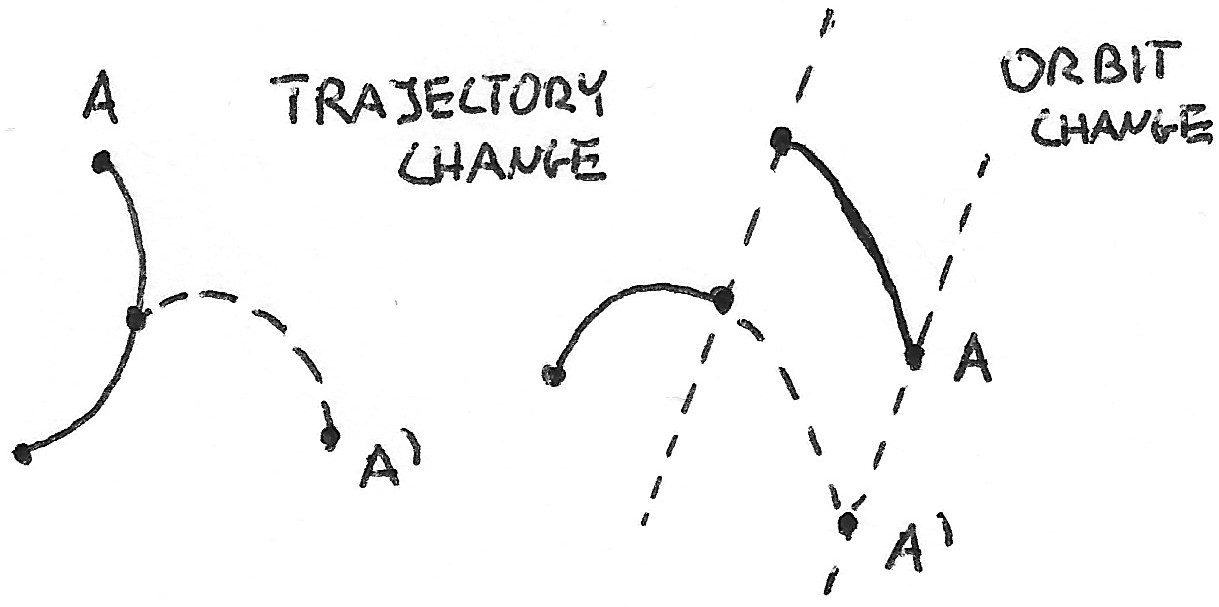
\includegraphics[width=6.25cm]{control-theory.jpeg}
  \caption{Changes in phase space. Point $A\prime$ represents the original destination, while $A$ chosen.}
  \label{fig:control-theory}
\end{figure}

Control theory is an interdisciplinary branch of engineering and mathematics that deals with the behavior of dynamical systems with inputs, and how their behavior is modified by feedback (figure \ref{fig:control-theory}). In our model, it will be a collection of operations which aims to control evolution function on the basis of input \cite{2006math......3133H}. Below example of \textit{Henon map}, in general sense $i$-th coordinate function $p_i$:

$$\displaystyle\begin{gathered}
\rnode[t]{TT}{\text{parameter}}\\\\
\rnode[b]{L}{p_i(\vec{x})} = 1 - \rnode[b]{T}{a} \rnode[b]{R1}{x_1^2} + \rnode[b]{R2}{x_2}\\[12pt]
\rnode[t]{LT}{\text{next $i$-th coordinate}}\qquad \rnode[t]{RT}{\text{previous coordinates}}
\psset{nodesep=2.5pt,arrows=->}
\ncline{L}{LT}\ncline{R1}{RT}\ncline{R2}{RT}
\ncline{T}{TT}
\end{gathered}$$

Each $p_i$ function modifies \textit{position} and may have own \textit{parameters}. Changing these variables will change phase space of this specific dynamical system. It can be done in two ways:

\begin{itemize}

\item\textbf{Orbit Change} (Position Change). This is done by selecting a new position, value $\vec{x}$, consequently changing the orbit. Then $i$-th dynamical system can be described as follows: $S_i = T^0_i(\vec{x})$.

\item\textbf{Trajectory Change} (Parameters Change). It involves selecting a new parameter values for $i$-th coordinate function $p_i$ of selected dynamical system from the buffer. In \textit{Henon map} it would be choosing new parameter $a$.

New parameters chosen for single transition function should be stored in \textit{parameters space} (section \ref{ssec:example-of-machine}). However, chosen parameters can be mutual with all transition functions in buffer. Then additional space is unnecessary.

\end{itemize}

\subsubsection{Hybrid System}
\label{sssec:hybrid-system}

\begin{figure}[ht]
  \centering
  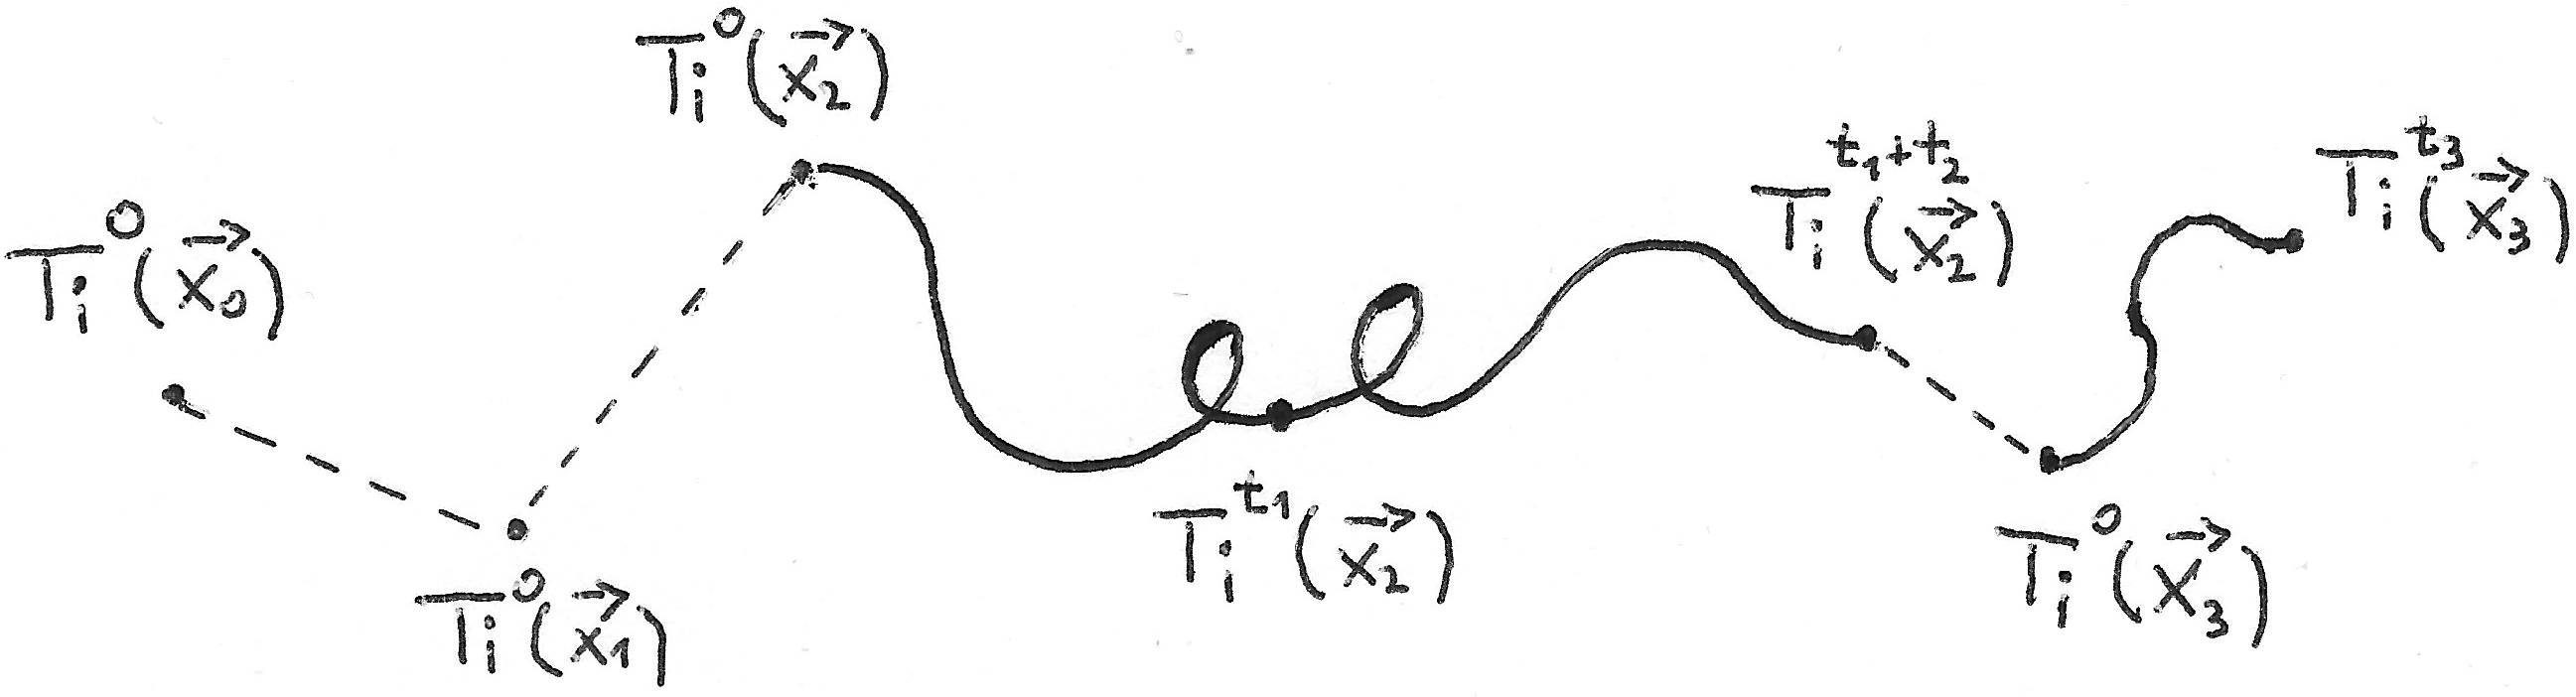
\includegraphics[width=9.25cm]{dynamical-system.jpeg}
  \caption{Phase space of $S_i$. Initial state $\vec{x_0} = \vec{k_i}$. Points $\{\vec{x_1}, \vec{x_2}, \vec{x_3}\}$ are selected by the push function - jumps. Pull function has evolved at $\{t_1, t_2, t_3\}$ time - flow.}
  \label{fig:hybrid-system}
\end{figure}

A hybrid system is a dynamic system that exhibits both continuous and discrete dynamic behavior - a system that can both ``flow'' described by a differential equation and ``jump'' described by a difference equation or control graph. In chaos machine, when performed (figure \ref{fig:hybrid-system}):

\begin{itemize}

\item\textbf{Push function} (chaotic), \textit{jumps} are governed by the collection of operations which aims to control evolution functions (section \ref{sssec:control-theory}). It modifies inflicted systems, based on initial secret key and input.

\item\textbf{Pull function} (random), \textit{flow} is governed by transition function $T$ that operates on buffer space. Its calculating evolution trace from the current position $\vec{x}$ of $S_i$: $$T^j_i(\vec{x}) \to T^{j+1}_i(\vec{x}) \to \dots \to T^{j+t}_i(\vec{x})$$

Where $j$ determines current time (\ref{dynamical-system} theorem), variable $t$ determines the length of time flow, known as \textit{time parameter}. After simplifications: $$S_i = T^{j+t}_i(\vec{x})$$

In addition, pull function may contain theorem of random dynamical system; equations of motion. Chaotic trajectories even look random, and they pass many classic ``tests of randomness''. This in fact generates the principle of equivalence between chaotic and random systems, as discussed in \cite{2013arXiv1310.1615W}.

\end{itemize}

%%%%%%%%%%%%%%%%%%%%%%%%%%%%%%%%%%%%%%%%%%%%%%%%%%%%%%%%%%%%%%%%%%%%%%%%%%%%%%%%%
%% PUSH FUNCTION

\subsection{Push Function}

Push function is primarily the input function of the machine, it absorbs bit string (typically 32 bits or 16 bits value, relatively small) and uses in system changes. The results are used later by the pull function. The push procedure is a collection of operations which aims to control evolution functions. It modifies inflicted systems, based on initial secret key and input. In summary, these ideas can be presented as:

\begin{itemize}

\item\textbf{Selection of Group}. Which systems from the buffer space should be changed (section \ref{sssec:buffer-space}).

\item\textbf{System Changes}. Controlling orbits and trajectories of selected dynamical systems - \textit{jumps} (section \ref{sssec:hybrid-system}).

\end{itemize}

Their implementation can be variously interpreted, that will be discussed in sections below. Fully implemented machine in \textit{python} programming language is in section \ref{ssec:example-of-machine}.

%%%%%%%%%%%%%%%%%%%%%%%%%%%%%%%%%%%%%%%%%%%%%%%%%%%%%%%%%%%%%%%%%%%%%%%%%%%%%%%%%
%% PULL FUNCTION

\subsection{Pull Function}
\label{sssec:pull-function}

The output of pull function is a bit string of fixed length (e.g., 16 or 32 bits), sequences of pseudo-random numbers that are unique and sensitive to the initial conditions. Push procedure contains 3 main tasks:

\begin{itemize}

\item\textbf{Selection of Group}. Which systems from the buffer space should be changed (section \ref{sssec:buffer-space}).

\item\textbf{System Evolution}. Calculating evolution trace of selected dynamical systems - \textit{flow} (section \ref{sssec:hybrid-system}).

\item\textbf{Randomizing}. Producing pseudo-randomness from chaotic data using pseudo-random functions.

\end{itemize}

%%%%%%%%%%%%%%%%%%%%%%%%%%%%%%%%%%%%%%%%%%%%%%%%%%%%%%%%%%%%%%%%%%%%%%%%%%%%%%%%%
%% INTERFACE
%%%%%%%%%%%%%%%%%%%%%%%%%%%%%%%%%%%%%%%%%%%%%%%%%%%%%%%%%%%%%%%%%%%%%%%%%%%%%%%%%

\section{Interface}

Goal for chaos machine is to make design that system designers can fairly easily incorporate into their own systems, and that is better at resisting the attacks we know about than the existing, widely-used alternatives. It poses the following constraints on the design of machine:

\begin{itemize}

\item Everything is reasonably efficient. There is no point in designing a module that nobody will use, because it slows down the application too much.

\item Machine is so easy to use that an intelligent, careful programmer with no background in cryptography has some reasonable chance of using it in secure way.

\item Interface should have simple design, to be able to implement many cryptographic primitives (figure \ref{fig:machine-applications}), including cryptographic hashes, message authentication codes, stream ciphers and pseudo-random number generators.

\end{itemize}

We found that the chaos machine can be compromised by exploiting some \textit{implementation error}. The only preventative measures we found for machine was to try to make the interface reasonably simple so that the programmer trying to use this tool in a real-world product can use it securely without understanding much about how the chaos machine works.

%%%%%%%%%%%%%%%%%%%%%%%%%%%%%%%%%%%%%%%%%%%%%%%%%%%%%%%%%%%%%%%%%%%%%%%%%%%%%%%%%
%% INPUT/OUTPUT

\subsection{Input/Output}

\begin{figure}
  \vspace*{2pt}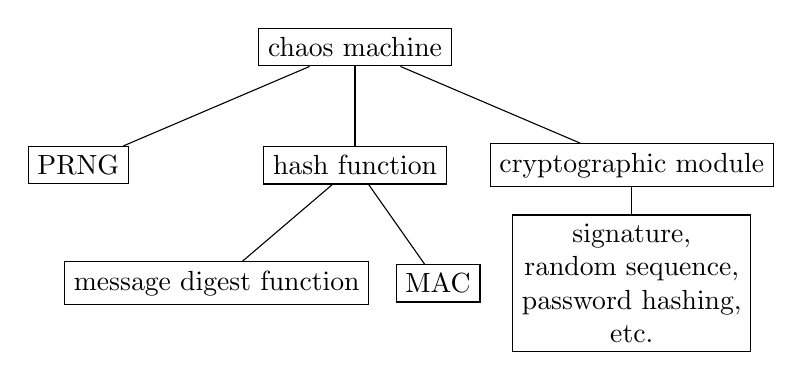
\begin{tikzpicture}[sibling distance=10em,
    every node/.style = {shape=rectangle,
      draw, align=center, color=black}]]
    \node {chaos machine}
      child { node {PRNG} }
      child { node {hash function}
        child { node {message digest function} }
        child { node [xshift=-2em] {MAC} } }
      child { node {cryptographic module}
        child { node {signature, \\random sequence, \\password hashing, \\etc.} } };
  \end{tikzpicture}
  \caption{Specially, numbers generated by chaos machine are useful in the following kinds of applications (interface and the parameters allow implementing).}
  \label{fig:machine-applications}
\end{figure}

As it was already mention (section \ref{ssec:concept}), chaos machine contains dynamical system of \textit{push-pull-reset functions} and \textit{buffer space}. These components are forming \textit{one-way} push-pull interface, making machine intuitively simple to use.

\begin{verbatim}
                // reset machine
                reset();

                // push to machine
                push(0xDEADBEAF);
                push(0xBADDCAFE);

                // pull a number
                uint32_t x = pull();

                // x = 0xB105F00D
\end{verbatim}

An important point which is worth to mention are the parameters, that regulates machine needs (section \ref{ssec:concept}). Number of iterations of the push and pull function is defined as the \textit{machine time}. In example above machine time amounts three (two push and one pull operation). A \textit{machine timeline} is a graphical representation of a period of machine time, on which push and pull events are marked (figure \ref{fig:interface-order}, \ref{fig:machine-types}).

%%%%%%%%%%%%%%%%%%%%%%%%%%%%%%%%%%%%%%%%%%%%%%%%%%%%%%%%%%%%%%%%%%%%%%%%%%%%%%%%%
%% STRUCTURE

\subsection{Structure}

Appropriate order of push and pull functions in time is called a construction or design. Programmer that is using the chaos machine can freely create his own designs. Often, it will be related to the application. If we have a message, we will have to perform some operations like push to add them to the machine. However, it may be done in many ways.

\subsubsection{Algorithmic Complexity}

Typically, if someone uses machine as hash function, he will push all data to machine and then pull message digest at the end. But he can pull after each push or according to another rule, making chaos machine applicable for \textit{stream hashing} or \textit{dynamical reseeding} (figure \ref{fig:interface-order}). For example let's imagine: \blockquote{We have an input 256 bits message and want to generate 512 bits of output. If machine operates on 32 bits input/output system, we must provide 256/32 = 8 push and 512/32 = 16 pull functions. It's worth to mention that attacker having an output, didn't know when at the timeline pull functions have been called, because he doesn't know the construction.} Computational complexity increase with the machine time. Number of possible combinations can be written as:

$$\binom{a + b}{b} * 2^{cb}$$\newline
Where variables are defined as: $a$ is a number of pull functions, $b$ is a number of push functions and $c$ is a number of bits per one input (if push operates on 16-bit blocks, $c = 16$).

\subsubsection{Types}

\begin{figure}[ht]
  \centering
  \begin{tabular}{l*{1}{l}r}
    Type & Relationship \\
    \hline
    Involved   & Input Data, Push \& Pull Sequence \\
    Individual & Input Data, Push Sequence
  \end{tabular}
  \caption{The table presents what influence the process of output generation.}
  \label{fig:table-types}
\end{figure}

\begin{figure*}[ht]
\begin{verbatim}
                  Case: #1
          time                   1        2        3        4        5        6        7
          interface            push() | push() | pull() | push() | pull() | pull() | pull()
          output                                   X                 X        X        X

                  Case: #2
          time                   1        2        3        4        5        6        7
          interface            push() | pull() | pull() | push() | push() | pull() | pull()
          output                          X        X                          X        X
\end{verbatim}
  \caption{Sequence of events plays a major role in output generation. Its management is held by the push-pull interface which creates a timeline of events. Input data pushed into machine in both cases is the same, parameters are the same, but output is different (same length, different sequences).}
  \label{fig:interface-order}
\end{figure*}

\begin{figure*}[ht]
\begin{verbatim}
                 Type: Involved
          time                1           2              3            4              5
          interface       push(X_1) | push(X_2) | pull() -> Y_1 | push(X_3) | pull() -> Y_3

          time                1           2                           3              4
          interface       push(X_1) | push(X_2) |    skipped    | push(X_3) | pull() -> Y_2

                 Type: Individual
          time                1           2              3            4              5
          interface       push(X_1) | push(X_2) | pull() -> Y_1 | push(X_3) | pull() -> Y_2

          time                1           2                           3              4
          interface       push(X_1) | push(X_2) |    skipped    | push(X_3) | pull() -> Y_2
\end{verbatim}
  \caption{Timeline above shows the difference between ``Involved'' and ``Individual'' type. Word ``skipped'' mean that none action was provided. In involved machine pull affects chaotic system (why value $Y_2 \neq Y_3$).}
  \label{fig:machine-types}
\end{figure*}

The \textit{butterfly effect}\footnote{It has similar properties to the \textit{avalanche effect}.} refers to a concept that small causes can have large effects. Consequently, pull function can be an event affecting future events and states. Therefore, there are two types of machines (figure \ref{fig:table-types}):

\begin{itemize}

\item\textbf{Involved}: The push function uses and modifies the states in the buffer. Each pull leans slightly\footnote{May contain theorem of random dynamical system, read more about \textit{pullback attractor}.} trajectories or orbits from buffer (butterfly effect in each event).

\item\textbf{Individual}: Push only reads states from the buffer or operates on copy. Therefore, after the same combination of push functions, pull gives the same sequence.

\end{itemize}

Visualization of difference between these types was presented at the figure \ref{fig:machine-types}. Sample example of involved type will be present in the part two of this document.

%%%%%%%%%%%%%%%%%%%%%%%%%%%%%%%%%%%%%%%%%%%%%%%%%%%%%%%%%%%%%%%%%%%%%%%%%%%%%%%%%
%% APPLICATION

\subsection{Application}

Chaos machine lets programmer to create own constructions and tools where \textit{randomness} and \textit{sensitiveness} is needed (figure \ref{fig:machine-applications}). Its presents modular design with customizable parameters. Where appropriate construction determines case of application, and where selection of parameters provides preferred properties and security level.

Practical example is provided in second part of this document. It includes sample implementation of chaos machine named Naive Czyzewski Generator, abbreviated NCG, that passes all the Dieharder, NIST and TestU01 test sets.

Below there will be analyzed the most typical applications. However, its recommend to use machine as an independent tool, due to the versatility and possibilities of use.

\subsubsection{Initialization Tuple}

The aim was to create a tool where user defines his needs by choosing appropriate parameters. For example, by selecting huge space parameter, machine produces long-period pseudo-random sequences\footnote{If period is calculable or can be approximate.}. Likewise, by increasing the time parameter, security level increases. Therefore, if security is a concern, chaos machine should fulfill these principles:

\begin{itemize}

\item Initial secret key should be provided or chosen uniformly.

\item Space parameter should be big enough to provide space-hardness and long-period output sequences.

\item Time parameter should be carefully selected to the appropriate level of security.

\end{itemize}

Slow one-way functions are useful as so-called password-based key derivation functions, where the relative high computation time protects against password guessing. The function can be made arbitrarily slow by increasing time parameter. In order to compete with fast pseudo-random number generators or speedy hash functions, machine should:

\begin{itemize}

\item Space parameter should be relatively small to the input data.

\item Time parameter must be very small or even equal to one iteration.

\end{itemize}

\subsection{Example of Machine}
\label{ssec:example-of-machine}

In \textit{python}, initialization tuple $(K, t, m)$ can be described as:

\begin{lstlisting}[style=codeAppendix, numbers=none]
# Chaos Machine (K, t, m)
K = [0.33, 0.44, 0.55, 0.44, 0.33]; t = 3; m = 5
\end{lstlisting}

\noindent Below example of chaos machine that is using \textit{Logistic map}\footnote{Its bad example, because its period is relatively small. The map itself has the characteristics unsuitable in cryptography.}: \begin{gather} p_1(\vec{x}) = r x_1 (1 - x_1) \\ T(\vec{x}) = T([x_1]) = [p_1] \\ S = \begin{bmatrix} T^0_1(\vec{k_1}) & T^0_2(\vec{k_2}) & T^0_3(\vec{k_3}) & T^0_4(\vec{k_4}) & T^0_5(\vec{k_5}) \end{bmatrix} \end{gather}

This map is one-dimensional, so it need only one coordinate function (3). Therefore, transition function $T$ looks like (4) and buffer space have 5 transition functions (5).

\subsubsection{Push Function}

In example below, push function is changing orbits and trajectories of all dynamical systems from buffer. Each system have own column in parameters space (for independent trajectory). In case above we are intrested in parameter $r$ that should be between 3 and 4 (chaotic behavior). Evolution parameter is variable that helps in controling evolution functions on the basis of input.

\begin{lstlisting}[style=codeAppendix, numbers=none]
# Buffer Space (with Parameters Space)
buffer_space, params_space = [], []

# Machine Time
machine_time = 0

def push(seed):
  global buffer_space, params_space, machine_time, \
    K, m, t

  # Choosing Dynamical Systems (All)
  for key, value in enumerate(buffer_space):
    # Evolution Parameter
    e = float(seed / value)

    # Control Theory: Orbit Change
    value = (buffer_space[(key + 1) % m] + e) % 1

    # Control Theory: Trajectory Change
    r = (params_space[key] + e) % 1 + 3

    # Modification (Transition Function) - Jumps
    buffer_space[key] =
      round(float(r * value * (1 - value)), 10)
    params_space[key] =
      r # Saving to Parameters Space

  # Logistic Map
  assert(max(buffer_space) < 1)
  assert(max(params_space) < 4)

  # Machine Time
  machine_time += 1
\end{lstlisting}

Pay attention, that buffer space is implemented as matrix of coordinate spaces ($n \times m$, where $n$ is number of space dimensions of transition function, or simpler, number of $p$ functions).

\subsubsection{Pull Function}

\begin{lstlisting}[style=codeAppendix, numbers=none]
def pull():
  global buffer_space, params_space, machine_time, \
    K, m, t

  # PRNG (Xorshift by George Marsaglia)
  def xorshift(X, Y):
    X ^= Y >> 13
    Y ^= X << 17
    X ^= Y >> 5
    return X

  # Choosing Dynamical Systems (Increment)
  key = machine_time % m

  # Evolution (Time Length)
  for i in range(0, t):
    # Variables (Position + Parameters)
    r     = params_space[key]
    value = buffer_space[key]

    # Modification (Transition Function) - Flow
    buffer_space[key] =
      round(float(r * value * (1 - value)), 10)
    params_space[key] =
      (machine_time * 0.01 + r * 1.01) % 1 + 3

  # Choosing Chaotic Data
  X = int(buffer_space[(key + 2) % m] * (10 ** 10))
  Y = int(buffer_space[(key - 2) % m] * (10 ** 10))

  # Machine Time
  machine_time += 1

  return xorshift(X, Y) % 0xFFFFFFFF
\end{lstlisting}

To generate pseudo-randomness, pull function use \textit{xorshift} algorithm with chaotic data. Additionaly, it includes \textit{pullback attractor} that leans trajectory of selected dynamical system.

\subsubsection{Reset Function}

\begin{lstlisting}[style=codeAppendix, numbers=none]
def reset():
  global buffer_space, params_space, machine_time, \
    K, m, t

  buffer_space = K; params_space = [0] * m
  machine_time = 0
\end{lstlisting}

Function above clears buffer, parameters space and resets machine time. After this, operation machine is in the initial state. It should be executed at the beginning of usage.

\vfill\eject

\subsubsection{Testing}

\begin{lstlisting}[style=codeAppendix, numbers=none]
# Initialization
reset()

# Pushing Data (Input)
import random
message = random.sample(range(0xFFFFFFFF), 100)
for chunk in message:
  push(chunk)

# Pulling Data (Output)
while True:
  print("%s" % format(pull(), '#04x'))
  print(buffer_space); print(params_space)
\end{lstlisting}

Implemented algorithm above is fully functional example of (involved) chaos machine, which has the characteristics of \textit{randomness} and \textit{sensitiveness}. This construction may not be producing a high-quality outputs. However, this example is using all theoretical knowledge about the chaos machine.

%%%%%%%%%%%%%%%%%%%%%%%%%%%%%%%%%%%%%%%%%%%%%%%%%%%%%%%%%%%%%%%%%%%%%%%%%%%%%%%%%
%%%%%%%%%%%%%%%%%%%%%%%%%%%%%%%%%%%%%%%%%%%%%%%%%%%%%%%%%%%%%%%%%%%%%%%%%%%%%%%%%
%% PART 2

\twocolumn[
  \begin{@twocolumnfalse}
  \clearpage
  \part{Naive Czyzewski Generator: Implementation of Chaos Machine}
  \vspace*{1.5cm}
  \end{@twocolumnfalse}
]

%%%%%%%%%%%%%%%%%%%%%%%%%%%%%%%%%%%%%%%%%%%%%%%%%%%%%%%%%%%%%%%%%%%%%%%%%%%%%%%%%
%% SUMMARY
%%%%%%%%%%%%%%%%%%%%%%%%%%%%%%%%%%%%%%%%%%%%%%%%%%%%%%%%%%%%%%%%%%%%%%%%%%%%%%%%%

\section{Summary}

The algorithm\footnote{This part was presented at the \textit{June 5, 2015}.} is a sample\footnote{The algorithm is not thoroughly discussed. If you want to know precisely how it works, please go to the section ``Appendix'' where is source code in ANSI C.} implementation of (involved) chaos machine. Emphasis has been placed on period that is calculable, but also on high sensitivity to initial conditions and quality of output. Algorithm passes all the Dieharder, NIST and TestU01 test sets. In addition, it shows resistance to common cryptographic attacks\footnote{Although it is ``designed to be cryptographically secure'', no security proof is given, and only statistical tests argue for its security.}.

\subsubsection{Disadvantages}

The drawback is the limited quantity of the machine parameters. On each push action, it engages all possible states from buffer space. Therefore, hashing for huge buffers does not make sense (computation complexity increase). When the buffer space is huge, the algorithm is suitable only for a use as the pseudo-random number generator. Therefore, it's has prefixed ``naive'' and instead of the word ``machine'' occurs ``generator''. However, for small values of parameters algorithm works as fully functioning chaos machine.

\subsubsection{Construction}

Transition function was constructed on modified logistic map. Buffer space is formed by the tape, which cells are grouped into two types. Pull function uses half of the cells by the algorithm with known period length (e.g. linear feedback shift register). The second half belongs to the set of dynamical systems. The only requirement is an even number of cells, in order to divide into equal halves. Therefore, variants are distinguished in the following way:

\begin{center}
  \begin{tabular}{lc}
    Name                         & Algorithm \\
    \hline
    $\text{NCG}$                 & LFSR  \\
    $\text{NCG}_{Xorshift}$      & Xorshift \\
    $\text{NCG}_{KISS}$          & KISS
  \end{tabular}
\end{center}

The examples above have been tested, in particular the basic version. However, they can be freely replaced.

\subsubsection{Security}

Statistical tests affirm that NCG can compete with ISAAC (as CSPRNG), Blum Blum Shub or Fortuna algorithm (figure \ref{result-tests}, \ref{result-rankit}, \ref{result-normal}). The NCG was designed and seems to be cryptographically secure, however there is no security proof.

\underline{Ten USA dollars prize} to whoever sends me the deterministic algorithm reconstructing seed/buffer space states from generated output sequence of pseudo-random numbers.

\begin{figure}[ht]
  \centering
  \begin{tabular}{lcr}
    Name of Battery & Total CPU Time & Result \\
    \hline
    Alphabit      & 00:00:00.03 & Passed \\
    SmallCrush    & 00:00:07.25 & Passed \\
    Crush         & 00:51:15.84 & Passed \\
    BigCrush      & 05:30:14.75 & Passed \\
    pseudoDIEHARD & 00:00:22.12 & Passed \\
    Rabbit        & 00:00:06.54 & Passed \\
    FIPS-140-2    & 00:00:12.24 & Passed
  \end{tabular}
  \caption{The result obtained using TestU01 (2.6 GHz Intel Core i7/clang v3.6.0). They were made for the algorithm presented in the ``Appendix'' section.}
  \label{result-tests}
\end{figure}

\begin{figure}[ht]
  \centering
  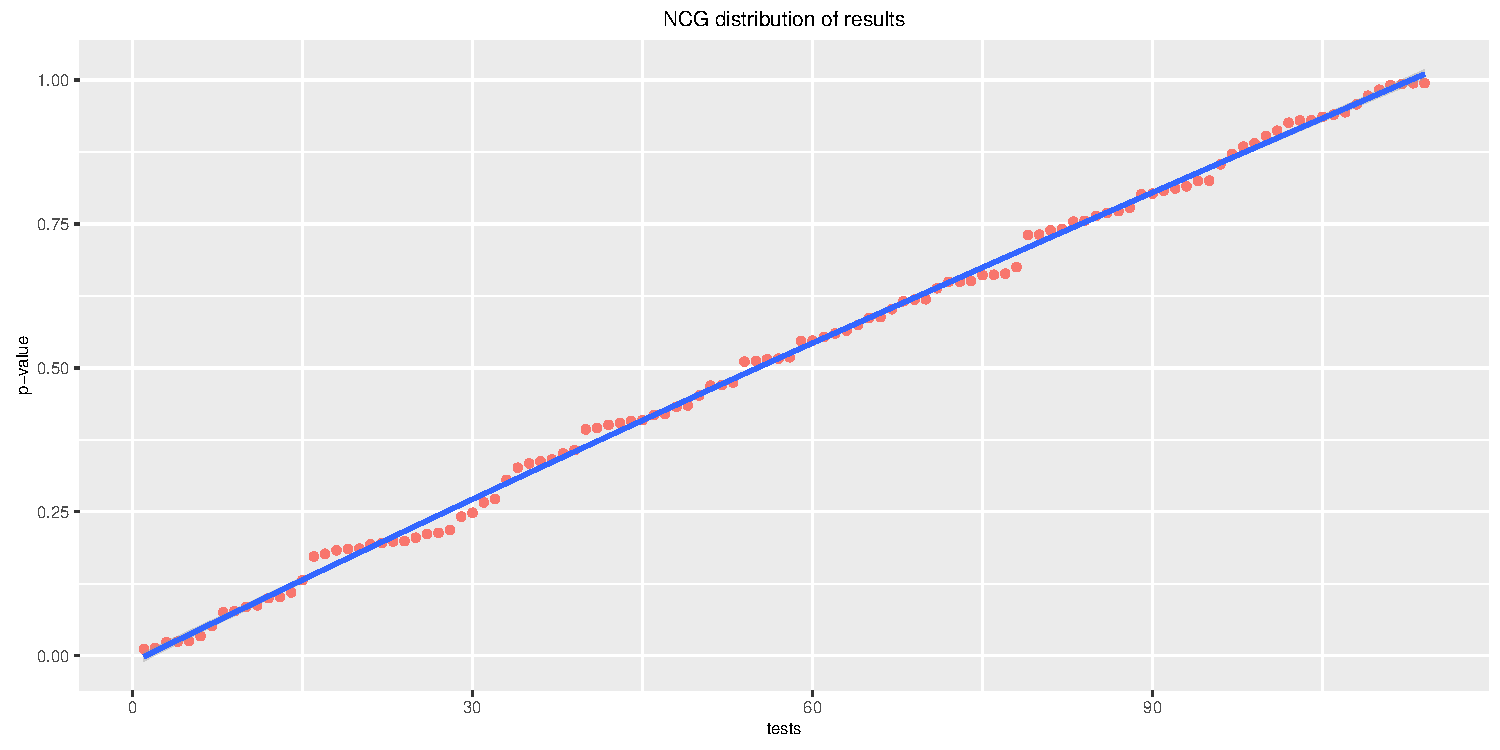
\includegraphics[width=9.25cm]{ncg-distribution-rankit}
  \caption{Normal probability plot (rankit), sorted p-values from statistical tests.}
  \label{result-rankit}
\end{figure}

\begin{figure}[ht]
  \centering
  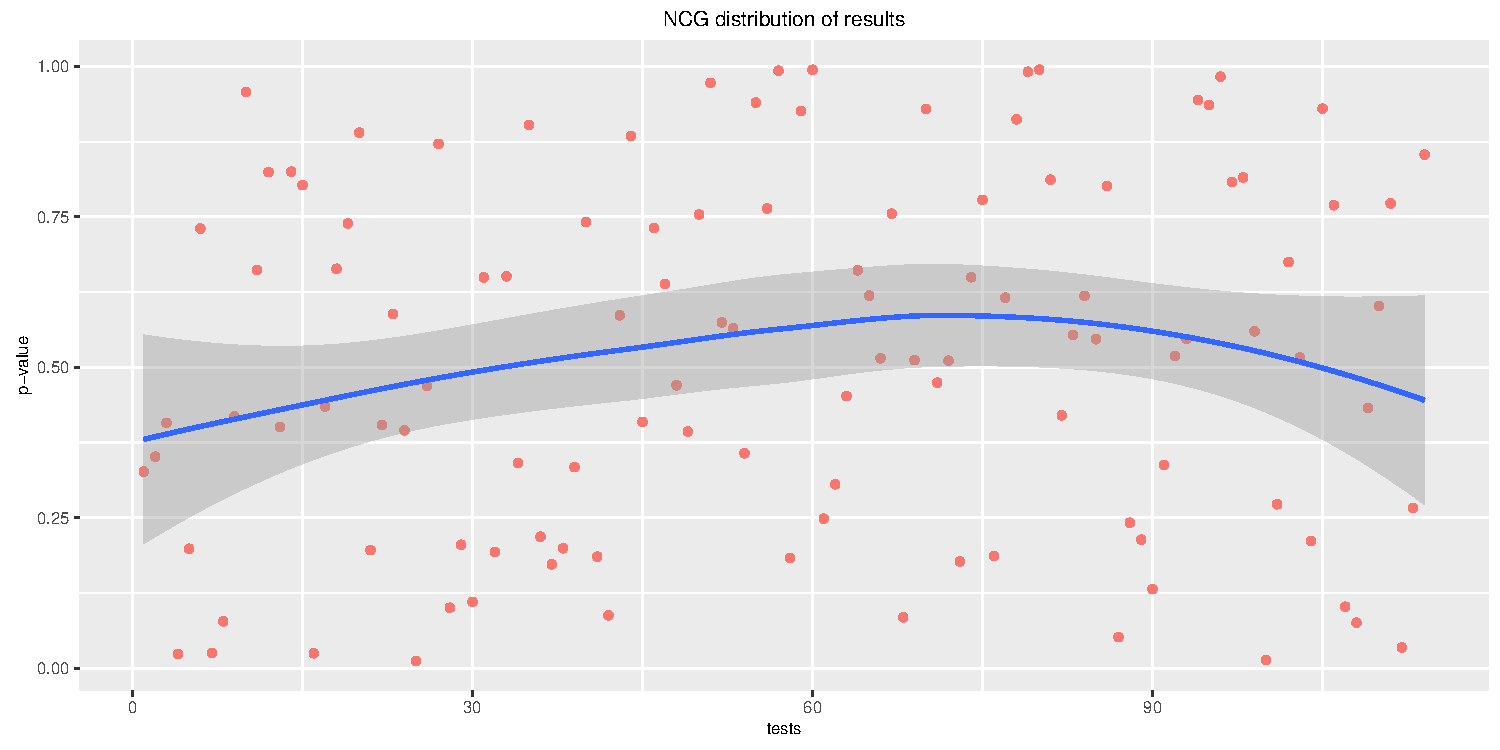
\includegraphics[width=9.25cm]{ncg-distribution-normal}
  \caption{Results of the Dieharder test sets in chronological order. An average p-value is 0.49 (blue line).}
  \label{result-normal}
\end{figure}

%%%%%%%%%%%%%%%%%%%%%%%%%%%%%%%%%%%%%%%%%%%%%%%%%%%%%%%%%%%%%%%%%%%%%%%%%%%%%%%%%
%% PARAMETERS
%%%%%%%%%%%%%%%%%%%%%%%%%%%%%%%%%%%%%%%%%%%%%%%%%%%%%%%%%%%%%%%%%%%%%%%%%%%%%%%%%

\section{Parameters}

The same parameters occur in the theoretical model of chaos machine. Additionally, in algorithm is located auxiliary function, it operates on the half of cells in the tape. Its task is to introduce cyclical fluctuations, in reference implementation it's LFSR\footnote{A linear-feedback shift register (LFSR) is a shift register whose input bit is a linear function of its previous state. The taps are XOR-ed sequentially with the rightmost bit and then fed back into the leftmost bit.} because its period is determined, but it can be changed to any other algorithm (table with variants).

\begin{figure}[ht]
  \centering
  \begin{tabular}{lcl}
    Parameter            & Value & Description \\
    \hline
    $\text{K}$           & $\pi$ digits & Initial secret key \\
    $\text{t}$ (TIME)    & 1            & Time parameter \\
    $\text{m}$ (SPACE)   & 16           & Space parameter
  \end{tabular}
  \caption{Above table of default parameters in algorithm. The requirement for $\text{m}$ is that it must be an even number.}
\end{figure}

\subsection{Time Parameter}

This parameter determines the number of rounds of computation that machine performs. The larger the time parameter, the longer the output computation will take. We make the exact time-space trade-offs precise on the figure \ref{result-benchmark}.

\begin{figure}[ht]
  \centering
  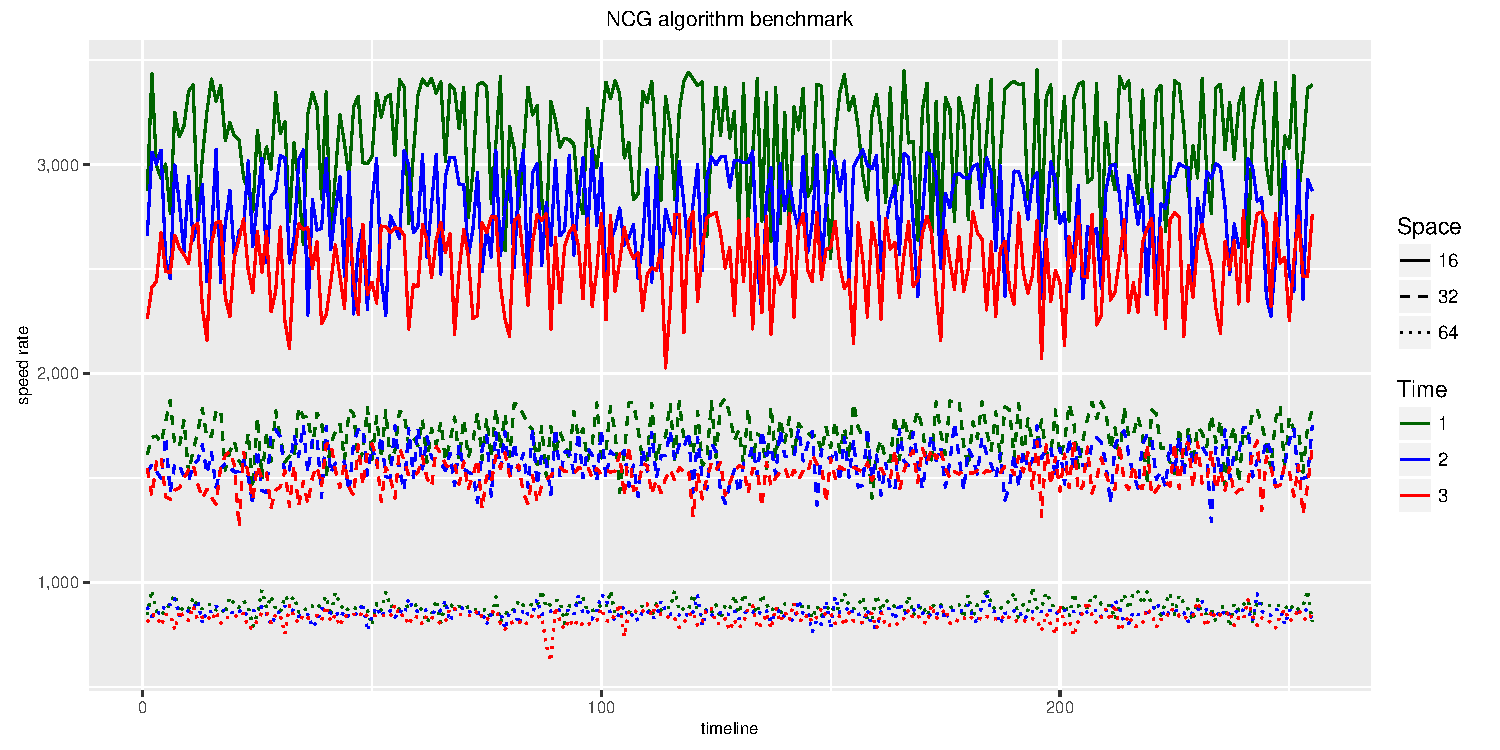
\includegraphics[width=9.50cm]{ncg-speed-benchmark}
  \caption{Plot that shows the impact of parameters to the speed rate. For each case, benchmark has performed 100,000 times the push and pull function with different input data. As we can see the algorithm slows 3 times for the 4 times bigger space parameter.}
  \label{result-benchmark}
\end{figure}

\subsection{Space Parameter}

In this machine, space parameter determines the length of the tape (number of cells). Let's assume that each cell has 16 bits capacity. Accordingly, half of the cells has a known\footnote{If a PRNG's internal state contains $n$ bits, its period can be no longer than $2^n$ results, and may be much shorter. LFSR have period $2^{n}$, but in this case cells have 16-bit, which gives period $2^{16}$.} period $2^{16}$, half unknown. It can be written as:

$$\prod^{\text{m}/2} 2^{16} \leq  x  \leq \prod^{\text{m}} 2^{16}$$
$$2^{8\text{m}} \leq  x  \leq 2^{16\text{m}}$$
$$2^{n/2} \leq  x  \leq 2^{n}$$

In the reference implementation we have $\text{m} = 16$, which gives the period $2^{128}$, which can be up to $2^{256}$. Hence, an implemented algorithm has a period between $2^{n/2}$ to $2^{n}$. Theoretically, if we have performed at every $2^{n/2}$ push function with truly random value, it will be possible to produce infinite period length.

%%%%%%%%%%%%%%%%%%%%%%%%%%%%%%%%%%%%%%%%%%%%%%%%%%%%%%%%%%%%%%%%%%%%%%%%%%%%%%%%%
%% APPLICATION
%%%%%%%%%%%%%%%%%%%%%%%%%%%%%%%%%%%%%%%%%%%%%%%%%%%%%%%%%%%%%%%%%%%%%%%%%%%%%%%%%

\section{Application}

Main aim of creating this algorithm was to present implemented model of chaos machine. As it was already mentioned before, the drawback is the limited quantity of the machine parameters. When the space parameter is huge, the algorithm is suitable only for a use as the PRNG.

At the beginning of the use of NCG, we must call the reset function. Initially, buffer space (entropy pool) is empty, but in accordance with the chaos machine model it must have an initial secret key. Code in ``Appendix'' is not thread safe.

\subsection{Pseudo-random Number Generator}

To implement generator we need to push seed into machine, and then pull out the pseudo-random numbers. Period is counted from the last execution of the push function, because there is no data from the outside (closed circuit). The same construction, input data and parameters will produce the same sequence of numbers, because the process is fully deterministic. However, with sufficient care, a system can be designed to produce cryptographically secure random numbers from the sources of randomness available in a modern computer. The basic design is to maintain an ``entropy pool'' of random bits that are assumed to be unknown to an attacker \cite{2014arXiv1412.7407O}. New randomness is added through push function to the buffer that evolves states of the machine.

\subsection{Hash Function}

The algorithm cannot compete with the speed of algorithms such as murmurhash3, farmhash or cityhash. However, the algorithm can be effectively used as a message authentication code where speed is not so important. Calculable period and excellent quality create narrow range of applications as hash function.

%%%%%%%%%%%%%%%%%%%%%%%%%%%%%%%%%%%%%%%%%%%%%%%%%%%%%%%%%%%%%%%%%%%%%%%%%%%%%%%%%
%% APPENDIX
%%%%%%%%%%%%%%%%%%%%%%%%%%%%%%%%%%%%%%%%%%%%%%%%%%%%%%%%%%%%%%%%%%%%%%%%%%%%%%%%%

\clearpage
\onecolumn

\section*{Appendix}

\subsection{Chaos Machine}

\begin{lstlisting}[style=codeAppendix]
/*  NCG written in 2015 by Maciej A. Czyzewski

To the extent possible under law, the author has dedicated all copyright
and related and neighboring rights to this software to the public domain
worldwide. This software is distributed without any warranty.

See <http://creativecommons.org/publicdomain/zero/1.0/>.  */

#include <stdint.h>
#include <string.h>

// S - seed, I - increment, t - mask, i - temporary
uint32_t S, I, t, i;

// The number of rounds in algorithm (time parameter)
#define TIME 1

// The length of the initial states (space parameter)
#define SPACE 16

// Abbreviation for getting values from the tape
#define M(i) ((i) % SPACE)

// Bits rotation formula
#define R(x, y) (((x) << (y)) | ((x) >> (16 - (y))))

// Variables in the algorithm
uint16_t a, b, c = 0, d = 0, e;

// Initial secret key - pi digits (buffer space)
uint16_t G[SPACE], K[SPACE] = { 1, 4, 1, 5, 9, 2, 6, 5,
                                3, 5, 8, 9, 7, 9, 3, 2 };

void push(uint32_t seed) {
  // Preparation
  I = seed * 0x3C6EF35F;

  for (S = seed, i = 0; i < SPACE; i++) {
    // Reinforcement
    G[M(i)] ^= ((I * (S + 1)) ^ S) >> 16;
    G[M(i)] ^= ((I * (S - 1)) ^ S) >> 00;

    // Finalization
    I ^= ((G[M(I - 1)] + G[M(i)]) << 16)
      ^  ((G[M(I + 1)] - G[M(i)]) << 00);
  }
}

uint32_t pull(void) {
  // Variables
  a = G[M(I + 0)]; b = G[M(I + 1)];

  // Initialization
  t = (a + I) * (b - S);

  // Chaos
  e = (G[M(t - b)] << (a % 9)) ^ (G[M(t + a)] >> (b % 9));

  // Rounds
  for (i = 0; i < TIME * 2; i += 2) {
    // Absorption
    c ^= G[M(I + i - 2)]; d ^= G[M(I + i + 2)];

    // Mixing                 Modification
    c ^= (d ^= R(e, c % 17)); G[M(I + i - 2)] -= (d += (t & c));
    d += (c += R(t, d % 17)); G[M(I + i + 2)] += (c += (e & d));
  }

  // Transition
  G[M(I + 0)] = R(c, t % 17) ^ R(d, t % 17) ^ (t & a) ^ (e & b);
  G[M(I + 1)] = (b >> 1) ^ (-(b & 1u) & 0xB400u); // LFSR

  // Finalization
  t += (c ^ (b << 8) ^ (d << 16) ^ (a & 0xFF) ^ ((a >> 8) << 24));

  // Cleaning
  c = d = 0xFFFF;

  // Increment
  I += 2;

  return t;
}

void reset(void) {
	// Copying defaults
	memcpy(G, K, 2 * SPACE);

	// Clearing parameters space
	c = d = 0x0000;

	// Initialized to non-zero values
	S = 0x19660D00;
	I = 0x3C6EF35F;
}
\end{lstlisting}

\subsection{Pseudo-random Number Generator}

\subsubsection{Implementation}

\begin{lstlisting}[style=codeAppendix]
void ncg(const uint32_t seed) {
  // Cleaning tape
  reset();

  // Push to NCG structure
  push(seed);
}
\end{lstlisting}

\subsubsection{Usage}

\begin{lstlisting}[style=codeAppendix]
#include <stdio.h>
#include <stdlib.h>

#include "../src/ncg.c"
#include "../src/include/random.c"

int main (int argc, char const *argv[])
{
  if (argc < 2) {
    printf("usage: %s <number> \n", argv[0]);
    return 1;
  }

  ncg((uint32_t) atoi(argv[1]));

  while (1) {
    putc_unlocked(pull(), stdout);
  }

  return 0;
}
\end{lstlisting}

\subsection{Hash Function}

\subsubsection{Implementation}

\begin{lstlisting}[style=codeAppendix]
#define GET_32_INT(n, b, i)                           \
{                                                     \
  (n) = ( (unsigned long) (b)[(i)    ]       )        \
      | ( (unsigned long) (b)[(i) + 1] << 8  )        \
      | ( (unsigned long) (b)[(i) + 2] << 16 )        \
      | ( (unsigned long) (b)[(i) + 3] << 24 );       \
}

#define PUT_32_INT(n, b, i)                           \
{                                                     \
  (b)[(i)    ] = (unsigned char) ( (n)       );       \
  (b)[(i) + 1] = (unsigned char) ( (n) >> 8  );       \
  (b)[(i) + 2] = (unsigned char) ( (n) >> 16 );       \
  (b)[(i) + 3] = (unsigned char) ( (n) >> 24 );       \
}

void ncg(const uint8_t *initial_message, size_t initial_length,
               uint8_t *result, size_t result_length) {
  // Cleaning tape
  reset();

  // Declaration of variables
  size_t length, offset;

  // Declaration of message
  uint8_t *message = NULL, *buffer = NULL;

  // Declaration of message chunk
  uint32_t chunk;

  // Calculate new length
  for (length = initial_length;
       length % 4 != 0; length++);

  // Prepare message
  message = (uint8_t*) malloc(length * 8);

  // Copy block of memory
  memcpy(message, initial_message, initial_length);

  // Complement to the full blocks
  if (length - initial_length > 0) {
    // Append "1" bit
    message[initial_length] = 0x80;

    // Append "0" bits
    for (offset = initial_length + 1; offset < length; offset++)
      message[offset] = 0;
  }

  // Append the len in bits at the end of the buffer
  PUT_32_INT(initial_length * 8, message + length, 0);

  // Initial_len >> 29 == initial_len * 8 >> 32, but avoids overflow
  PUT_32_INT(initial_length >> 29, message + length + 4, 0);

  // Process the message in successive 32-bit chunks
  for (int i = 0; i < length; i += 4) {
    // Get little endian
    GET_32_INT(chunk, message + i, 0);

    // Push to NCG structure
    push(chunk);
  }

  // Releasing memory
  free(message);

  // Allocate memory for result
  buffer = (uint8_t*) malloc(result_length * 8);

  // Process the result in successive 32-bit chunks
  for (int i = 0; i < result_length / 4 + 1; i++)
    PUT_32_INT(pull(), buffer, i * 4);

  // Save it on the pointer
  for (int i = 0; i < result_length; i++)
    result[i] = buffer[i];

  // Releasing memory
  free(buffer);
}
\end{lstlisting}

\subsubsection{Usage}

\begin{lstlisting}[style=codeAppendix]
#include <stdio.h>
#include <stdlib.h>

#include "../src/ncg.c"
#include "../src/include/hash.c"

int main (int argc, char const *argv[])
{
  const char *initial_message = argv[1];
  size_t initial_length = strlen(initial_message);

  if (argc < 3) {
    printf("usage: %s 'string' <number> \n", argv[0]);
    return 1;
  }

  size_t result_length = atoi(argv[2]);
  uint8_t *result = (uint8_t*) malloc(result_length * 8);

  printf(">> ");
  for (int i = 0; i < initial_length; i++)
    printf("%p ", initial_message[i]);
  printf("\n");

  ncg((uint8_t*) initial_message, initial_length, result, result_length);

  printf("<< ");
  for (int i = 0; i < result_length; i++)
    printf("%p ", result[i]);
  printf("\n");

  return 0;
}
\end{lstlisting}

%%%%%%%%%%%%%%%%%%%%%%%%%%%%%%%%%%%%%%%%%%%%%%%%%%%%%%%%%%%%%%%%%%%%%%%%%%%%%%%%%
%% BIBLIOGRAPHY
%%%%%%%%%%%%%%%%%%%%%%%%%%%%%%%%%%%%%%%%%%%%%%%%%%%%%%%%%%%%%%%%%%%%%%%%%%%%%%%%%

\clearpage
\onecolumn

\printbibliography[title={References}]

%%                               END OF DOCUMENT                               %%
%%%%%%%%%%%%%%%%%%%%%%%%%%%%%%%%%%%%%%%%%%%%%%%%%%%%%%%%%%%%%%%%%%%%%%%%%%%%%%%%%
%%%%%%%%%%%%%%%%%%%%%%%%%%%%%%%%%%%%%%%%%%%%%%%%%%%%%%%%%%%%%%%%%%%%%%%%%%%%%%%%%

\end{document}
